\documentclass[11pt,a4paper]{scrartcl}
\typearea{12}
\usepackage{graphicx}
\usepackage{pstricks}
\usepackage{listings}

\usepackage{tikz}
\usepackage{amsmath}



\tikzset{
    state/.style={
           rectangle,
           rounded corners,
           draw=black, very thick,
           inner sep=2pt,
           text centered,
           },
}
\tikzset{
    on/.style={
           circle,
           draw=red, very thick,
           inner sep=2pt,
           fill=red!25,
           },
}


\tikzset{
    off/.style={
           circle,
           draw=blue, very thick,
           inner sep=2pt,
           text centered,
           },
}



\lstset{language=python}
\pagestyle{headings}
\markright{PHPHM0017 - 2 synapses - Conor Houghton}

\begin{document}

\subsection*{Chemical synapses}

Spikes, the voltage pulses that carry signals from neuron to neuron,
are notably stereotypical; there aren't big spikes and small spikes,
to a good approximation, there are just spikes. However, the effect
one neuron has on the other can vary considerably, not just from
neuron to neuron, but from time to time. This variablity can occur
because of chemical synapses, the complicated biochemical machinery
responsible for connect the axon of one neuron to the dendrite of
another. 

Chemical synapses are not the only synapses, there are also
\textsl{gap junctions}. If an axon is connected to a dendrite by a gap
junction there is a small hole directly connecting the inside of one
neuron through to the inside of the other, usually this means that the
axon of one neuron is connected to the dentrite of the other, though
axon to axon gap junctions are also found. For an axon to dentrite gap
junction this means that when a spike travelling along the axon
reaches the gap junction some of the charged ions diffuse through the
gap changing the charge in the dendrite. In some simple animals like
jelly fish most or all of the synapses are gap junctions. There are
gap junctions in the mammalian brain, for example gap junctions are
thought to be responsible for the dynamics which supports very rapid
oscillations in the hippocampus, however, most of the synapses in the
mammalian brain are chemical synapses. We will see that this allows a
more variable effect of a pre-synaptic spike on the voltage of the
post-synaptic dendrite.

In a chemical synapse the pre-synaptic spike does not affect the
post-synaptic voltage directly, instead it causes a cascade of
bio-electrodynamics events which ultimately causes a transient change
in conductance of the post-synaptic membrane. 

Roughly, the synapse consists of a protuberance in the axon called the
\textsl{terminal bouton}, the terminal bouton is held by astrocytes,
supporting non-neuronal brain cells, so that it is separated by a tiny
gap, called the \textsl{synaptic cleft} from a protuberance in the
dendrite called the \textsl{dendritic spine}; depending on the neurons
involved this protuberance might be a small bump, or a substantial
spine The shape of the spine is thought to be important in the
modulation of synaptic signalling; this isn't an aspect of synapses we
will consider here.


The terminal bouton is filled with tiny bags or bubbles called
\textsl{vesicles}, these contain special molecules called
\textsl{neurotransmitters}. When a spike arrives at the terminal
bouton it causes calcium gates to open in the cellular membrane, the
resulting influx of calcium ions causes some of the vesicles to
migrate to the membrane separating the bouton from the synaptic cleft,
they burst releasing neurotransmitter into the cleft.

\begin{figure}
      \begin{center}
      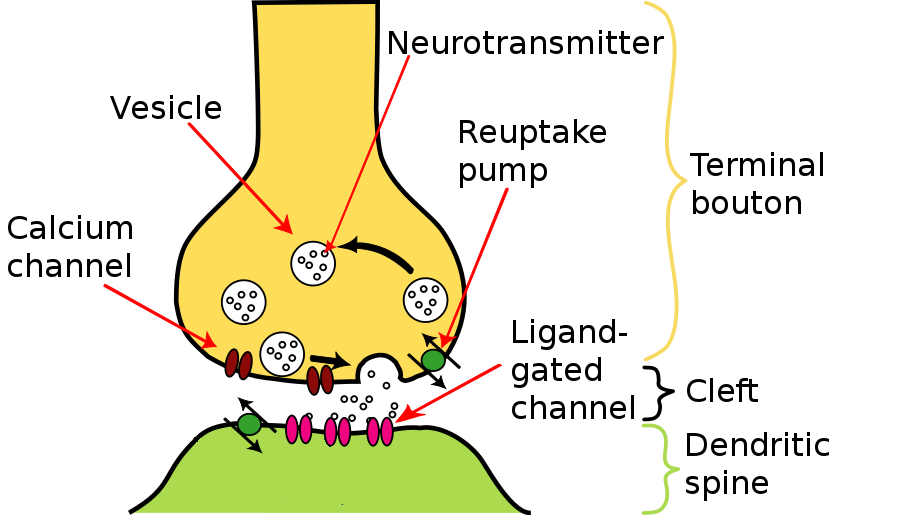
\includegraphics[width=12cm]{Synapse.png}
      \end{center}
\caption{The major parts of the synapse; this shows a vesicle
  bursting, releasing neurotransmitter into the cleft, this will bind
  with the ligand-gated channels to allow a current across the
  membrane of the dendrite. Reuptake pumps are shown in the bouton and
  the spine, there are also pumps in the astrocyte that surrounds the
  cleft but isn't shown here. Some is also lost to diffusion. [Diagram
    modified from one in wikipedia.]}
\end{figure}

The membrane of the dendritic is pieced by gated ion channels; these
are \textsl{ligand gated} channels. This means that they contain a
receptor site which binds with a particular type of molecule, like a
key designed for the receptor site's lock. When the receptor has a
molecule bound to it, the gate is open and so ions can pass through
the channel, like the other channels we have seen the channel is ion
specific, so only one type of ion can pass through it. In the case of
the ligand-gated channels in the dendritic spine, the neurotransmitter
binds with the receptor, opening the gate. Hence, after a spike
arrives at the synapse the cleft is filled with neurotransmitter and
some of that neurotransmitter binds to the gated channels, causing
them to open. This in turn allows a flow of ions in or out of the
dendrite, changing the voltage there.

Which ion and which direction, depends on the synapses, we will return
to that. For now, though, let us continue describing what happen;
after the neurotransmitter floods the cleft it is quickly reabsorbed
through neurotransmitter reuptake pumps. Some of the neurotransmitter
is absorbed into the bouton, some into the spine and some is absorbed
by the astrocyte, the important thing is that the concentration of
neurotransmitter in the cleft falls rapidly. Now, the fluid of the
cleft has little neurotransmitter, but there is still neurotransmitter
bound to the receptors of the ligand gated channels. This gradually
unbinds, this is usually imagined to be a random process, because of
the Brownian motion of molecules in the fluid of the cleft and the
thermal vibration of the receptor itself, the neurotransmitters unbind
as the result of random collisions and thermal variations. As they do
so, the channels close again and the conductivity of the dendritic
spine's membrane falls back towards zero.

\subsection*{Post-synaptic potential}

One important property of neurons is that a given neuron is either
\textsl{excitatory} or \textsl{inhibitory}. If a neuron is excitatory,
this means all its synapses are excitatory, that is, they make the
post-synaptic neuron more likely to spike by increasing its
voltage. In an excitatory neuron opening the ligand-gated channels
causes a positive current into the cell, typically this means that
they are sodium or calcium channels, so that when they open positive
sodium or calcium ions flow into the dendrite. Conversely, if a neuron
is inhibitory all its synapses are inhibitory, they make the
post-synaptic cell less likely to fire by decreasing its voltage. In
an inhibitory synapse opening the ligand-gated channels causes a
positive flow out of the dendrite, lowering the voltage. Typically
inhibitory channels are either potassium gates, allowing postive
potassium to leave the dendrite, or chlorine gates, allowing
negatively charged chlorine to flow in.

The post-synaptic change in potential that results from a pre-synaptic
spike is called a \textsl{post-synaptic potential}; if the synapse is
excitatory this is called an \textsl{excitatory post-synaptic
  potential} or EPSP, if it is inhibitory it is called an
\textsl{inhibitory post-synaptic potential} or IPSP. The profile of
PSPs reflects the neurotransmitter dynamics, it rises fast as the
neurotransmitter floods the cleft and the ion-channels open, it then
decays back to zero following an exponential decay, reflecting the
constant rate unbinding process: since any bound molecule has a
constant probability of shaking free the number of unbinding events
depends on the number of bound molecules, giving an exponential decay.

From a modeling point of view all this means that there is a current
corresponding to the synapse:
\begin{equation}
I_s(t)=g_s(t)(E_s-V)
\end{equation}
where $g_s(t)$ is the conductance at the synapse and $E_s$ is the
reversal potential for whichever ion the synapse conducts, for an
excitatory synapse this might be the reversal potential for sodium so
that $E_s$ is perhaps 20 mV, for an inhibitory neuron it might be
potassium with $E_s=-80$ mV, for example. The next part of the model needs to describe the dynamics of $g_s(t)$. For convenience we often write
\begin{equation}
  g_s=\bar{g}_ss(t)
\end{equation}
where $\bar{g}_s$ is the overall strength and $s(t)$ is the bit that
changes with time. The simplest model is probably one that ignores any
detail of the rapid process of vesicle release and binding, it also
ignores any interaction between spikes, the possibility some channels
might already have bound to a neuro-transmitter, or that the calcium
in the synapse may have accumulated or that the vesicles may have
depleted.

In this simplified situation the synapse model only accounts for the
gradual closing of the channels as they unbind from the
neurotransmitter and the sudden increase of open channels whenever a
spike arrives. In this model the equation is just
model the conductance as
\begin{equation}
\tau_s\frac{ds}{dt}=-s
\end{equation}
with
\begin{equation}
s(t)\rightarrow s(t)+p
\end{equation}
whenever there is a spike, where $p$ is a constant, often taken as
one.



\end{document}
